\documentclass[t, english]{beamer}
\usetheme{Frankfurt}
\usepackage[utf8]{inputenc}
\usepackage{natbib}
%\usepackage[french]{babel}
\usepackage[english]{babel}
\usepackage{listings}
\usepackage{hyperref}
\usepackage{tikz}
\usepackage{algorithm}
\usepackage[noend]{algpseudocode}
\usepackage{pgfplots}
\usepackage{comment}

%animations (for gifs)
\usepackage{animate}

%customize itemize
\usetikzlibrary{positioning,calc,intersections,shapes.geometric}

\setbeamertemplate{footline}[frame number]


%New commands for the SSA form
\newcommand{\ssa}[1]{\begin{align*}#1\end{align*}}
\newcommand{\cst}{\textit{cst}}
\newcommand{\readstate}{\textit{read-state}}
\newcommand{\setstate}{\textit{set-state}}
\newcommand{\exectask}{\textit{exec-task}}
\newcommand{\apply}{\textit{apply}}


\title{ICAPS - IntEx 2022}
\subtitle{Guidance of a Refinement-based Acting Engine with a Hierarchical Temporal Planner}
\author{Jérémy Turi, Arthur Bit-Monnot \\
jeremy.turi@laas.fr, abitmonnot@laas.fr}
\institute{LAAS-CNRS}
\date{\today}

\begin{document}

\begin{frame}
\titlepage
\end{frame}

\begin{frame}
\frametitle{Outline}
\tableofcontents
\end{frame}

\AtBeginSection[]
{
  \begin{frame}
    \frametitle{Table of Contents}
    \tableofcontents[currentsection]
  \end{frame}
}

\begin{comment}
\begin{frame}{Goal of the presentation}
  The goal of the presentation is to present an agent with autonomous deliberation capabilities, able to make wise decisions thanks to look-ahead techniques.
\end{frame}
\end{comment}



\section{Deliberative agent (7 min)}

\begin{frame}{What is an agent}

    \begin{columns}[T]
        \begin{column}{0.3\textwidth}
            A robotic agent

            ~

            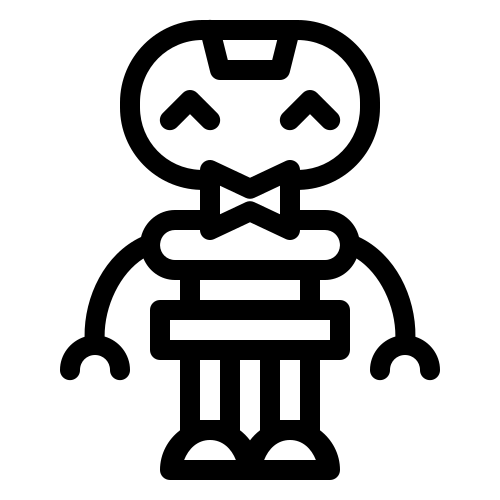
\includegraphics[width = 0.7\textwidth]{images/icons8-robot-gustav-500.png}
        \end{column}
        \begin{column}{0.7\textwidth}
            \center capable of :
            \pause
            \begin{enumerate}
                \item Perceiving its environment
                \pause
                \item Modifying its environment (actions)
                \pause
                \item \textbf{Deliberating:} Reasoning about its \textbf{skills} in order to fulfill a goal
            \end{enumerate}
        \end{column}
    \end{columns}

 
\end{frame}

\begin{frame}{Represent the skills of an agent}

\begin{columns}[T]
    \begin{column}{0.6\textwidth}

        Robot behavior = \textbf{operational model}:
        \begin{itemize}
            \item Executable program
            \item General purpose language
        \end{itemize}
        
        ~

        
        Acting domain \textbf{$A_\Delta (A, T, M_t)$}: Hierarchical operational models
        
                \begin{itemize}
        
        
         \item[$A$] \textit{(low-level skills)}: primitive tasks
         \pause
         
         \textit{\footnotesize(move, grasp, look)}
         \pause
         \item[$T$] \textit{(high-level skills)}: abstract tasks
         \pause

         \textit{\footnotesize(set the table, prepare a coffee)}
         \pause
         \item[$M_t$] \textit{("Know how")}: methods (operational models)

         
     \end{itemize}
    \end{column}
    \begin{column}{0.45\textwidth}
        \begin{figure}
            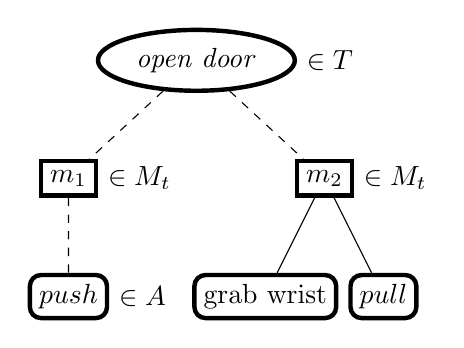
\begin{tikzpicture}
                \node[draw,ellipse, ultra thick] (t) {\textit{open door}} [sibling distance = 3.25cm]
                  child {node[draw, ultra thick] (m1) {$m_1$} edge from parent [dashed]
                  child {node[draw,rounded corners, ultra thick, solid] (a1) {$push$} edge from parent
                  }} 
                  child {node[draw, ultra thick] (m2) {$m_2$} edge from parent [dashed] [sibling distance = 1.5cm]
                  child {node[draw, rounded corners, solid, ultra thick] (a2) {grab wrist} edge from parent [solid]}
                  child {node[draw, rounded corners, solid, ultra thick] {$pull$} edge from parent [solid]}};
                \node[right = 0em of t] {$\in T$};
                \node[right = 0em of m1] {$\in M_t$};
                \node[right = 0em of m2] {$\in M_t$};
                \node[right = 0em of a1] {$\in A$};

            \end{tikzpicture}
            \caption{Example of hierarchy for the \textit{task} \textit{open door}}

            
        \end{figure}
    \end{column}
\end{columns}
    
\end{frame}
\begin{frame}{Refinement Acting Engine (RAE)\cite{ghallabAutomatedPlanningActing2016} : Deliberation algorithms using hierarchical operational models}
\begin{columns}
    \begin{column}{0.35\textwidth}
    \pause
    \setlength{\leftmargini}{-1pt}
    %\setlength{\parsep}{1pt}
    %\setlength{\parskip}{0pt}
    RAE features:
    \small
    \begin{itemize}
        \item Perform multiple tasks in parallel
        \pause
        \item Automated deliberation: Refinement of task
        \begin{itemize}
            \setlength{\leftmargini}{-1pt}
            \pause
            \item Refinement of task into a method
            \pause
            \item Instantiating of \textbf{arbitrary} variables
        \end{itemize}
    \end{itemize}
    \end{column}
    \begin{column}{0.65\textwidth}
        Algorithms:
        \small
        \begin{itemize}
            \setlength{\leftmargini}{-1pt}
            \item \textbf{Main:} 
            \begin{itemize}
                \item Receive $\tau$ (task or event);
                
                add it to the \textbf{agenda} (ongoing tasks)
                \pause
                \item Refine $tau$: \textbf{Select} an applicable method $m$ for $\tau$
                \pause
                \item \textbf{Progress} $m$
            \end{itemize}
            \item \textbf{Progress:}
                \begin{itemize}
                \item Monitor execution of $m$.
                \item Refine subtasks in $m$.    
                \item Monitor execution of subtasks.
                \item \textbf{Retry} $\tau$ in case of \emph{failure}:
                
                Call \textbf{Select} to get a new method;
                
                \textbf{Progress} the new method.
                \end{itemize}
                \pause
        \end{itemize}
    \end{column}
\end{columns}

    
\end{frame}

\begin{frame}{Improve the refinement using planning}
    \begin{center}
        
    Role of Select:

    ~

    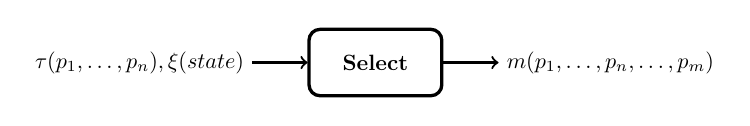
\begin{tikzpicture}[thick,scale=0.8, every node/.style={scale=0.8}]
    \node[draw = black, very thick,
        minimum width = 6em,
        minimum height = 3em,
        rounded corners,
        text = black,
        align=center,] (F) at (0,0) {\textbf{Select}};
        
    \pause
    \node[left= 2em of F] (i) {\textbf{$\tau(p_1,\dots,p_n), \xi (state)$}};
    \node[right= 2em of F] (o) {\textbf{$m(p_1, \dots, p_n,\dots,p_m)$}};
    \pause
    \path[->]
    (i) edge (F)
    (F) edge (o);

    \end{tikzpicture}
    

    %$Select(\tau, p_1,\dots,p_n) \rightarrow \{m_s, p_1, \dots, p_n,\dots,p_m\}$

    \end{center}

    Techniques:
    \begin{itemize}

    \item Greedy (Basic RAE functioning): arbitrary applicable method
    \pause
    
    \underline{Problem:} Does not take into account future refinements (can lead into dead-locks)
    \pause
    \item \textbf{look-ahead(planning)} : capacity to project the system from the current state to possible future state

    \end{itemize}
\end{frame}
\begin{frame}{How to use planning in RAE}
    %Make a high-level choice based on future choices the agent will have to make and its own capabilities to modify its environment.
    Requires:
    \begin{itemize}
        \item A planner
        \item Descriptive model of the agent skills : describes the set of states that may result from performing tasks.
    \end{itemize} 

    Descriptive models shortcomings:
    \begin{itemize}
        \item Made limited dedicated languages: PDDL \cite{foxPDDL2ExtensionPDDL2003}, ANML \cite{smith2008anml},\dots
        \item operational model $\not\equiv$ descriptive model $\rightarrow$ Harder design
    \end{itemize}

    ~
    
    \centering
    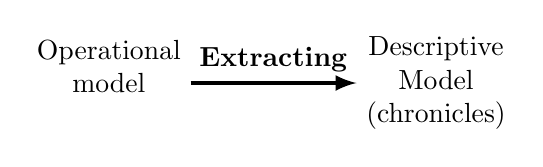
\begin{tikzpicture}
        \node[align = center] (O) {Operational\\ model \\};
        \node[right=6em of O, align = center] (D) {Descriptive\\ Model \\(chronicles)};
        \draw[-latex, ultra thick] (O.east)-- node[above, midway] (c) {\textbf{Extracting}} (D.west);
    \end{tikzpicture}

    Plan with \textbf{Aries} (hierarchical LCP\cite{bit-monnotConstraintBasedEncodingDomainIndependent2018} extension):

\end{frame}

\begin{frame}[c]{An analyzable acting language to extract descriptive models}
    \begin{columns}[c]
        \begin{column}{0.45\textwidth}
            Acting language Requirements:
            \begin{itemize}
                \item General purpose language
                \item Identified and simple semantic
            \end{itemize}
        \end{column}
        \begin{column}[c]{0.1\textwidth}
            \centering
            $\rightarrow$
        \end{column}
        \begin{column}{0.5\textwidth}
            Lisp dialect (Scheme variant) \cite{moretti1979lambda}

            Perks:
            \begin{itemize}
                \item Few primitives
                \item Immutable
                \item Functional
                \item Pure
            \end{itemize}
        \end{column}
    \end{columns}
\end{frame}

\begin{frame}{Synthesis of the proposition}
    \pause
        \centering
        Task refinement guided by planning:

        ~
        
        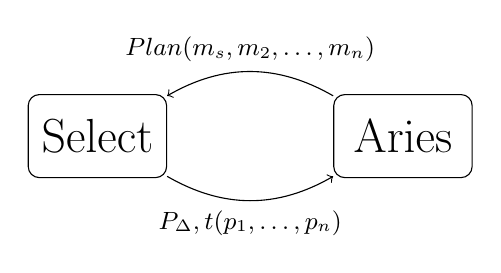
\begin{tikzpicture}
            \node[draw,
            rounded corners,
            minimum width = 5em,
            minimum height = 3em] (select) {\LARGE Select};
            \node[draw,
            rounded corners,
            right = 6em of select,
            minimum width = 5em,
            minimum height = 3em] (aries) {\LARGE Aries};
            \path[->, every node/.style={font=\sffamily\small}]
            (select) edge[bend right] node [right, below] {$P_\Delta, t(p_1,\dots,p_n)$} (aries)
            (aries) edge[bend right] node [right, above] {$Plan(m_s, m_2,\dots,m_n)$} (select)
            ;
        \end{tikzpicture}

        ~
    
        Planning domain extraction from operational models:

        ~

        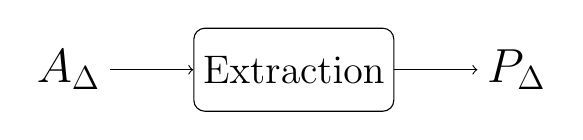
\begin{tikzpicture}
            \node (acting) {\LARGE $A_\Delta$};
            
            \node[draw,
            rounded corners,
            right= 3em of acting,
            minimum height = 3em,
            minimum width = 6em] (ext) {\Large Extraction};
        
            \node[right = 3em of ext] (planning) {\LARGE $P_\Delta$ };
            
            \path[->, every node/.style={font=\sffamily\small}]
            (acting) edge (ext)
            (ext) edge (planning);
          \end{tikzpicture}

\end{frame}



\section{RAE for multi-agent systems}
\subsection{Operational Model Planning and Acting System}

\begin{frame}{The Operational Model Planning and Acting System (OMPAS), an extension to RAE}
    \begin{columns}[t]
        \begin{column}{0.5\textwidth}
    New \textbf{task} in \textbf{dedicated thread}
    \begin{figure}
        \tikzstyle{thread} = [draw, rounded corners, rectangle, fill=black!50]
    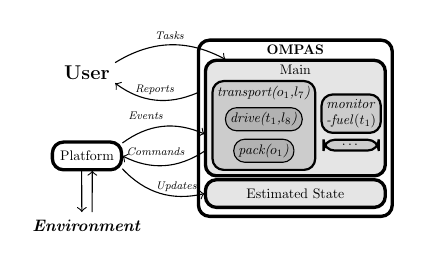
\begin{tikzpicture}[scale=0.5, every node/.style={scale=0.5}]
  
        %RAE
        \node[draw = black, very thick,
            minimum width = 14em,
            minimum height = 5em,
            rounded corners,
            text = black,
            text centered, text depth = 4 cm,
            align = center,
            ] (R) at (0,0) {\textbf{OMPAS}};
        %Operational Models
        % \node[draw = black, ellipse, very thick,
        %     minimum width = 7em,
        %     minimum height = 2em,
        %     above = 1em of R,
        %     text = black,
        %     text centered, align=center
        % ] (OM) {\textit{Operational Models} %($A_\Delta$)
        % };
  
  
        %state
        \node[draw = black, very thick,
        text centered,
        minimum width = 13em,
        minimum height = 2em,
        rounded corners,
        text = black,
        fill=black!10,
        align = center] (S) at ($(R.south) + (0,0.6)$) {Estimated State};
  
        %main
        \node[draw = black, very thick,
        minimum height = 8em,
        minimum width = 13em,
        rounded corners,
        text = black,
        text centered, text depth = 7em,
        fill=black!10,
        align=center] (main) at ($(R.north) + (0,-2)$) {Main};
  
        %t1
        \node[draw = black, thick,
        minimum height = 6em,
        minimum width = 7em,
        rounded corners,
        text = black,
        text centered, text depth = 5em,
        fill=black!20,
        align=center](t1) at ($(main.south) + (-0.8, 1.3)$) {\emph{transport($o_1$,$l_7$)}};
  
  
        %first task
        \node[draw, rounded corners, rectangle, fill=black!30] (st11) at ($(t1.south) + (0,1.3)$) {\emph{drive($t_1$,$l_8$)}};
        \node[draw, rounded corners, rectangle, fill=black!30] (st12) at ($(st11.south) + (0,-.5)$){\emph{pack($o_1$)}};
        
        \node[draw, thick, rounded corners, rectangle,minimum width = 4em, fill=black!20, align= center] (t3) at ($(t1.east) + (0.9, 0.3)$){\textit{monitor}\\
        \textit{-fuel}($t_1$)};
        \node[draw, thick, rounded corners, rectangle,minimum width = 4em, fill=black!20, align= center] (t3) at ($(t1.east) + (0.9, -0.5)$){\dots};
  
  
  
        %platform
        \node[draw = black, very thick,
        text centered,
        minimum width = 5em,
        minimum height = 2em,
        %below = 2em of R,
        rounded corners,
        text = black,
        align = center,] (Pl) at ($(R.west) +(-8em, -2em)$) {Platform};
  
        \node[text centered,
        minimum width = 5em,
        minimum height = 2em,
        below = 1.5em of Pl,
        rounded corners,
        text = black,
        align = center,] (E) {\textbf{\large\textit{Environment}}};
  
        \node[very thick,
            text centered,
            rounded corners,
            text = black] (U) at ($(R.west) +(-8em, +4em)$) {\Large \textbf{User}};
        
        % \node[draw = black, very thick,
        %     text centered,
        %     right = 7em of R,
        %     minimum width = 5em,
        %     minimum height = 4em,
        %     rounded corners,
        %     text = black] (Pl) {Platform};
        
  
        \path[->]
  
            %Link between operational models library
            %(OM) edge (R)
  
            (U.20) edge[bend left] node [midway, above, align=center] {\footnotesize \emph{Tasks}} (main.+140)
            (R.+160) edge [bend left] node [midway, above] {\footnotesize \emph{Reports}} (U.-20)
        
            %Link between RAE and the platform
            (main.-160) edge[bend left] node [pos = 0.6, above = 0.2em] {\footnotesize \emph{Commands}} (Pl.east)
            
            %between platform and state
            (Pl.-20) edge [bend right] node [pos = 0.7, right, above, align = center] {\footnotesize \emph{Updates}} (S.west)
            
            %between platform and main
            (Pl.20) edge [bend left] node [pos = 0.3, right, above= 0.2em, align = center] {\footnotesize \emph{Events}} (main.-170)
  
            (Pl.-110) edge (E.110)
            (E.70) edge (Pl.-70)
            ;
        
        \end{tikzpicture}
        \caption{Overview of OMPAS architecture}
    \end{figure}
            
        \end{column}
        \pause
        \begin{column}{0.5\textwidth}
        Operational language with
        \begin{itemize}
            \item \textbf{Acting} features
            \item \textbf{Generic} programming constructs
            \item First-hand concurrency support (interruption, resource)
            \item \textbf{Simple semantic} $\rightarrow$ \textbf{guide} the \textbf{acting choices} with \textbf{automated analysis} of \textbf{skills}
        \end{itemize}
        \end{column}
    \end{columns}
\end{frame}

\subsection{Acting language}

\begin{frame}[fragile]{SOMPAS: A Lisp variant based on Scheme}
    \centering
    Scheme : Recursive evaluation of \textbf{expressions} \verb|(f e1 ... en)|
    
    ~~

\pause
    \begin{columns}[t]
        \begin{column}{0.65\textwidth}
            Definitions:
            \begin{itemize}
                \item \textbf{Expression} = \{Atom, List of expression\}
                \item \textbf{Atom} = \{Symbol, Boolean, Number, Procedure\}
            \end{itemize}
\pause
        \end{column}
        \begin{column}{0.35\textwidth}
            Scheme \textbf{advantages}:
            \begin{itemize}
                \item Few primitives
                \item Functional
                \item \textbf{Simple to extend}
            \end{itemize}
        \end{column}
     \end{columns}
\end{frame}

\begin{frame}[fragile]{Acting primitives}
    \begin{columns}
        \begin{column}{0.5\textwidth}
            Functions:
            \begin{itemize}
                \pause
                    \item \textbf{\textit{(exec a $p_1...p_n$)}} executes and monitors a task or command.
                    % \begin{itemize}
                    %     \item command : resorts to the platform
                    %     \item task: selects a method and execute its operational model.
                    % \end{itemize}
                \pause
                    \item \textbf{\textit{(read-state sf $p_1...p_n$)}} returns the value of a state-variable
                % \pause
                %     \item \textit{(arbitrary set $\lambda$)} returns an arbitrary element from a $set$%. $\lambda$ can be used to select among the $set$.
                \end{itemize}
        \end{column}
    \pause
        \begin{column}{0.5\textwidth}
               
        Example:
    \small
        \lstset{columns=fullflexible}
        \begin{lstlisting}[language = lisp]
    (begin
        (define loc-p (read-state loc ?p))
        (define loc-r (read-state loc ?r))
        (if (!= loc-p loc-r)
            (exec move ?r loc-p))
        (exec pick ?r ?p) 
        (exec move ?r ?l)
        (exec place ?r ?p))             
        \end{lstlisting}
        \end{column}
    \end{columns}
    \end{frame}


\begin{frame}[fragile]{Scheme extension for concurrency and interruption}

    Definition of a new Atom: the \emph{handle}
    
    ~~
\pause
    \begin{columns}
        \begin{column}{0.6\textwidth}
            Functions:
            \begin{itemize}
                \item \textbf{\textit{(async e)}}: creates a new thread to evaluate e, returns a handle
                \item \textbf{\textit{(await h)}}: awaits the result of the concurrent evaluation.
                \item \textbf{\textit{(interrupt h)}}: interrupts the concurrent evaluation.
                \item \textbf{\textit{(uninterruptible e)}}: prevent interruption signals.
            \end{itemize}
        \end{column}
        \pause
        \begin{column}{0.4\textwidth}
        Example: 
\small
\lstset{columns=fullflexible}
            \begin{lstlisting}[language = lisp]
(begin
    (define h1 (async (+ 1 2)))
    (define h2 (async (* 3 3)))
    (+ (await h1) (await h2)))
-> 12 
            \end{lstlisting}
        \end{column}
    \end{columns}
\end{frame}

\begin{frame}[fragile]{Example of program with interruptions.}
    
\begin{columns}
    \begin{column}{0.4\textwidth}
        \lstset{basicstyle=\footnotesize, columns=fullflexible}
\begin{lstlisting}[language=lisp]
(begin
 (define h
  (async 
    (begin
     (uninterruptible (begin
       (exec pick ?r ?o)
       (exec move ?r ?l)
       (exec drop ?r ?o)))
     (exec inspect ?r ?o))))
 (race 
   (await h)
   (begin
    (sleep 10)
    (interrupt h))))
\end{lstlisting}

    \end{column}
    \begin{column}{0.6\textwidth}
        \newcommand{\Cross}{$\mathbin{\tikz [x=1.4em,y=1.4em,line width=.2em, red] \draw (0,0) -- (1,1) (0,1) -- (1,0);}$}
    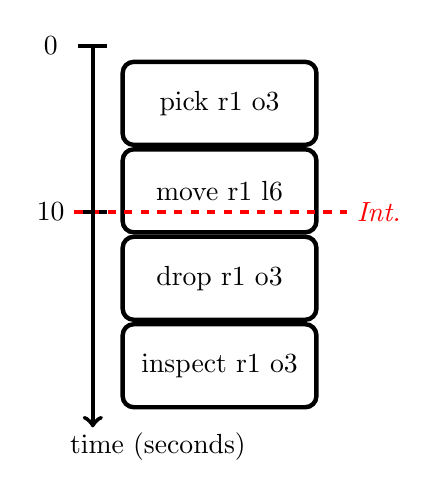
\begin{tikzpicture}
        \node[draw,
        rounded corners,
        ultra thick,
        minimum height = 3em,
            minimum width = 7em,] (pick) at (0,0) {pick r1 o3};
    
        \node[draw, rounded corners,
        ultra thick,
            minimum height = 3em,
            minimum width = 7em,
        ] (move) at ($1.5*(pick.south)-0.5*(pick.north)$) {move r1 l6};
        %\action{move, move r1 l6, 10em, pick}
    
        \node[draw, rounded corners,
        ultra thick,
            minimum height = 3em,
            minimum width = 7em,
        ] (drop) at ($1.5*(move.south) - 0.5*(move.north)$) {drop r1 o3};
        \node[draw, rounded corners,
        ultra thick,
            minimum height = 3em,
            minimum width = 7em,
        ] (inspect) at ($1.5*(drop.south) - 0.5*(drop.north)$) {inspect r1 o3};
        \node at (inspect) {\Cross};
    
            \node[] (origin) at ($(pick.north west) + (-1em,+0.5em)$) {~~};
        
            \node[] (zero) at ($(origin.west) + (-1em,0)$) {0};
            \draw[-, ultra thick] (origin.west) -- (origin.east);
            \node[] (ten) at ($(zero) + (0,-6em)$) {10};
            \draw[-, ultra thick] ($(origin.west) + (0,-6em)$) -- ($(origin.east) + (0,-6em)$);
    
    
            \node[] (interruption) at ($(ten.east) +(11em,0em)$){\color{red} \textit{Int.}};%{\color{red} \textit{interruption}};
            \draw[-, ultra thick, dashed, color= red] ($(ten.east)$) -- ( interruption);
            \node[] (end) at ($1.5*(inspect.south west) - 0.5*(inspect.south west) + (-1em,-1em)$) {};
            \node[] (time) at ($1.5*(end.south east) - 0.5*(end.south east) + (2em,0)$)  {time (seconds)};
    
    
        \path[->] (origin.center) edge[ultra thick] (end);
    \end{tikzpicture}
    \end{column}
\end{columns}    
\end{frame}


\begin{frame}[fragile]{Resource model for safe concurrent execution}
    Definition of a resource:
    \begin{columns}
        \begin{column}{0.5\textwidth}
            \begin{itemize}
                \item Object \textbf{r} with initial capacity $C(0) = C_{init} $
                \item Acquire($r$,$c$) at time $t$ $\implies$ $c \leq C(t)$ 
            \end{itemize}
        \end{column}
        \pause
        \begin{column}{0.5\textwidth}
            \begin{itemize}
                \item \textbf{\textit{unary}:} $C_{init} = 1, c = 1$;
                \item \textbf{\textit{divisible}}: $C_{init} \in  \mathbb{R}_+^*, c \in ]0, C(t)]$
            \end{itemize}
        \end{column}
    \end{columns}
    
    ~~

\pause
    \begin{columns}
        \begin{column}{0.6\textwidth}
            Functions:
            \begin{itemize}
                \item \textbf{\textit{(new-resource r C)}} : create a new resource $r$ with capacity $C$
                \item \textbf{\textit{(acquire r c)}} : acquisition request for $r$ with amount $c$, returns a resource handle
                \item \textbf{\textit{(release h)}} : release the resource using the resource handle
            \end{itemize}
        \end{column}
        \pause
        \begin{column}{0.4\textwidth}
        Example: 
            \small
            \lstset{columns=fullflexible}
            \begin{lstlisting}[language = lisp]
(begin
 (new-resource r1)
 ...
 (define hr (acquire r1))
 (exec move r1 x y)
 (release hr)
)
            \end{lstlisting}
        \end{column}
    \end{columns}
\end{frame}

% \begin{frame}{More advanced features and programming constructs}
%     More complex behavior definition
%     \begin{itemize}
%         \item \textit{(wait-for dyn)} waits until the expression \textit{dyn} becomes true 
%         \item \textit{(run-monitoring e dyn)} evaluates \textit{e} while \textit{dyn} is true, interrupts \textit{e} otherwise.
%         \item ...
%     \end{itemize}
% \end{frame}

% \begin{frame}[t,fragile]{Defining an acting domain with SOMPAS}
%     \setlength{\leftmargini}{0pt}
%     \begin{columns}
%         \begin{column}{0.5\textwidth}
%             \begin{itemize}
%                 \footnotesize
%                 \item Task (label, typed parameters):
%                 \tiny
%                 \begin{lstlisting}
% (def-task t_process_package
%     (:params (?p package)))
%                 \end{lstlisting}
%                 \footnotesize
%                 \pause
%                 \item Method (label, typed parameters, pre-conditions, body):
%                 \tiny
%                 \begin{lstlisting}
% (def-method m_process_to_do_r
%   (:task t_process_package)
%   (:params (?p package))
%   (:pre-conditions
%     (!= (package.processes_list ?p)
%         nil)))
%   (:body
%     (do
%      (define ?m ...)
%      (t_process_on_machine ?p ?m)
%      (t_process_package ?p)))   
%                 \end{lstlisting}
%             \end{itemize}
%         \end{column}
%     \pause
%         \begin{column}{0.5\textwidth}
%             \begin{itemize}
%     \pause
%             \footnotesize
%             \item State-function (label, typed parameters \& result):
%             \tiny
%             \begin{lstlisting}
% (def-state-function at
%     (:params (?r robot))
%     (:result location))
%             \end{lstlisting}
%     \pause
%             \footnotesize
%             \item Command (label, typed parameters):
%             \tiny
%             \begin{lstlisting}
% (def-command pick (:params (?r robot)))
%                 \end{lstlisting}
%             \end{itemize}

%     \pause
%             ~
%         \normalsize
%         Others:
        
%         \textit{lambda, type, constant}
%         \end{column}

%     \end{columns}
% \end{frame}


%\section{RAE+Planning (6min)}
\subsection{Improving Select algorithm of RAE}
\begin{frame}
    Goal: Improve high-level choices quality taking into account future choices and primitives tasks models.
\end{frame}
\begin{frame}{Select-Plan}
    
\end{frame}
\begin{frame}{Extraction of the planning domain}
    
\end{frame}
\begin{frame}{Enhancement of the chronicles with post processing}
    
\end{frame}
\begin{frame}{Primitive task models}
    
\end{frame}
\begin{frame}{Validation of the technique: gripper-door}
    \begin{itemize}
        \item Global view on the problem
        \item Acting domain
    \end{itemize}
\end{frame}
\begin{frame}{Results}
    
\end{frame}
\begin{frame}{Analysis and critics}
    
\end{frame}
\section{Conclusion \& perspectives (2 min)}
\begin{frame}{On the paper}
    
\end{frame}
\begin{frame}{Perspectives}
    
\end{frame}
\begin{frame}[allowframebreaks]
  \frametitle{References}
  \bibliographystyle{plain}
  \bibliography{biblio}
\end{frame}


\end{document}
